\documentclass[titlepage]{article}
\usepackage{babel}
\usepackage{amsmath}
\usepackage{amssymb}
\usepackage{amsthm}
\usepackage{multicol} %spalten in seite
\usepackage{graphicx} %bilder einfügen
\usepackage[normalem]{ulem} %durchstreichen
\usepackage{tabto} %tabulator mit \tab
\usepackage{hyperref}
\usepackage{tikz}
\usetikzlibrary{shapes.geometric}
\usepackage{wasysym}
\usepackage{bbm}
\usepackage{bbold}
\usepackage{xcolor}
\usepackage[T1]{fontenc}
\usepackage{mathrsfs}  
\usepackage[utf8]{inputenc}
\usepackage{listings} %quellcode
\pagestyle{plain}
\pagenumbering{arabic}
\renewcommand{\arraystretch}{1.3} %vertikaler abstand von tabellen
\newcommand{\n}{\newline}
\usepackage[left=20mm, right=15mm, top=25mm, bottom=7mm, paper=a4paper]{geometry}
\renewcommand{\contentsname}{Inhaltsverzeichnis}

\newcommand{\K}{\mathbb{K}}
\newcommand{\C}{\mathbb{C}}
\newcommand{\N}{\mathbb{N}}
\newcommand{\Q}{\mathbb{Q}}
\newcommand{\R}{\mathbb{R}}
\newcommand{\1}{\mathbb{1}}
\newcommand{\0}{\mathbb{0}}
\newcommand{\Z}{\mathbb{Z}}

\begin{document}
	
	\begin{center}
		
\begin{tikzpicture}
			\draw (0,0) node[draw, rectangle]{\textsc{Wintersemester 2020/21}};
		\end{tikzpicture}
		\hrulefill\\
		\begin{center}
			\LARGE\textsc{Diskrete Strukturen - Übung 09} \normalsize\\
		\end{center}
		\hrulefill
		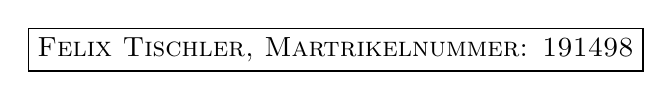
\begin{tikzpicture}
			\draw (0,0) node[draw, rectangle]{\textsc{Felix Tischler, Martrikelnummer: 191498}};
		\end{tikzpicture}
		\date{\today}
	\end{center}

	\subsection*{Kreuzprodukt}
		\subsubsection*{$1.)$}
			\begin{table}[h]
				\begin{tabular}{clcl}
					$(a)$&$(A\cap B)\times C$ $=$ $(A\times C)\cap(B\times C)$&
					$(d)$&$(A\cup B)\times(C\cup D)$ $\supseteq$ $(A\times C)\cup(B\times D)$\\
					$(b)$&$(A\cup B)\times C$ $=$ $(A\times C)\cup(B\times C)$&
					$(e)$&$(A\times B)\cap(C\times D)$ $=$ $(A\cap C)\times(B\cap D)$\\
					$(c)$&$(A\cap B)\times(C\cap D)$ $=$ $(A\times C)\cap(B\times D)$&
					$(f)$&$(A\times B)\cup(C\times D)$ $\subseteq$ $(A\cup C)\times(B\cup D)$
				\end{tabular}
			\end{table}
		Begründung:
			\begin{align*}
				(a)\quad&(A\cap B)\times C=\{(x,y)\mid x\in(A\cap B)\land y\in C\}=\{(x,y)\mid x\in A\land x\in B\land y\in C\}=(A\times C)\cap(B\times C)\qed
				\\
				(b)\quad&(A\cup B)\times C=\{(x,y)\mid x\in(A\cup B)\land y\in C\}=\{(x,y)\mid x\in A\lor x\in B\land y\in C\}=(A\times C)\cup(B\times C)\qed
				\\
				(c)\quad&(A\cap B)\times(C\cap D)=\{(x,y)\mid x\in (A\cap B)\land y\in(C\cap D)\}=\{(x,y)\mid x\in A\land x\in B\land y\in C\land y\in D\}\\&=(A\times B)\cap(C\times D)\qed
				\\
				(d)\quad&(A\cup B)\times(C\cup D)=\{(x,y)\mid x\in(A\cup B)\land y\in (C\cup D)\}=\{(x,y)\mid x\in A\lor x\in B\land y\in C\lor y\in D\}\\&\supseteq\{(x,y)\mid x\in A\land y\in B\lor x\in C\land y\in D\}=\{(x,y)\mid (x,y)\in(A\times C)\lor(x,y)\in(B\times D)\}\\&=(A\times C)\cup(B\times D)\qed
				\\
				(e)\quad&(A\times B)\cap(C\times D)=\{(x,y)\mid (x,y)\in(A\times B)\land(x,y)\in(C\times D)\}=\{x\in A\land\ y\in B\land x\in C\land y\in D\}\\&=\{(x,y)\mid x\in(A\cap C)\land y\in(B\cap D)\}=(A\cap C)\times(B\cap D)\qed
				\\
				(f)\quad&(A\times B)\cup(C\times D)=\{(x,y)\mid(x,y)\in(A\times B)\lor(x,y)\in(C\times D)\}=\{(x,y)\mid x\in A\land y\in B\lor x\in C\land y\in D\}\\&\subseteq\{(x,y)\mid x\in A\lor x\in C\land y\in B\lor y\in D\}=\{(x,y)\mid x\in(A\cup C)\land y\in(B\cup D)\}\qed
			\end{align*}
		
	\subsection*{Relationen}
		\subsubsection*{$2.)$}
			\begin{table}[h]
				\begin{tabular}{clclclcl}
					$(\alpha)$&\textit{a ist Schwester von b.}&
					$(\beta)$&\textit{a ist Mutter von b.}&
					$(\gamma)$&\textit{a ist Enkel von b.}&
					$(\delta)$&\textit{a ist Großmutter von b.}\\
					$(\varepsilon)$&\textit{a ist Schwester von b.}&%mit einer weiteren
					$(\zeta)$&\textit{a ist Tochter von b.}&%mit weiterer schwester
					$(\eta)$&\textit{a ist Nichte von b.}&
					$(\theta)$&\textit{a ist die Mutter von b.}%mit weiterer Tochter
				\end{tabular}
			\end{table}
		
		\subsubsection*{$3.)$}
			\paragraph{$(a)$}
				Seien $R\subseteq A\times B$ und $S\subseteq B\times C$, dann ist $R\circ S=_{df}\{(a,b)\mid\underset{S\in B}{\bigvee}((a,b)\in R\land(b,c)\in S)\}\subseteq A\times C\qed$
			\paragraph{$(b)$}\scalebox{1}{
				$x\,(R\circ S)\circ T\,y\leftrightarrow x\,R\circ S\,k\land k\,T\,y\leftrightarrow x\,R\,f\land f\,S\,k\land k\,T\,y\leftrightarrow x\,R\,f\land f\,S\circ T\,y\leftrightarrow x\,R\circ (S\circ T)\,y$\qed}
			\paragraph{$(c)$}
				$(x\,R\,y\land x\,S\,y)\circ T\leftrightarrow (x\,R\,w\land w\,T\,y)\land(x\,S\,t\land t\,T\,y)\leftrightarrow R\circ T\cap S\circ T\qed$
				
				
			\paragraph{$(d)$}\scalebox{1}{
				$x\,(R\circ S)^{-1}\,y\leftrightarrow y\,(R\circ S)\,x\leftrightarrow y\,R\,g\land g\,S\,x\leftrightarrow g\,R^{-1}\,y\land x\,S^{-1}\,g\leftrightarrow x\,S^{-1}\,g\land g\,R^{-1}\,y\leftrightarrow x\,S^{-1}\circ T^{-1}\,y$\qed}
\end{document}
